\documentclass[12pt, twoside]{article}
\usepackage[letterpaper, margin=1in, headsep=0.5in]{geometry}
\usepackage[english]{babel}
\usepackage[utf8]{inputenc}
\usepackage{amsmath}
\usepackage{amsfonts}
\usepackage{amssymb}
\usepackage{tikz}
\usetikzlibrary{quotes, angles}
\usepackage{venndiagram}
\usepackage{multicol}

\usepackage{fancyhdr}
\pagestyle{fancy}
\fancyhf{}
\renewcommand{\headrulewidth}{0pt} % disable the underline of the header

\fancyhead[RE]{\thepage}
\fancyhead[RO]{\thepage \\ Name: \hspace{3cm}}
\fancyhead[L]{BECA / Dr. Huson / IB Math\\* 1 December 2020}


\begin{document}
\subsubsection*{2.10 Final exam: Measure, trigonometry}
All answers should be exact or rounded to three significant figures.

\begin{enumerate}

\item A cylinder has a radius of 3.1 cm and height of 11.4 cm. 
  \begin{enumerate}
    \item Calculate the volume of the cylinder. \hfill (2 marks)
    \item Find the total surface area of the cylinder. \hfill (2 marks)
  \end{enumerate}

\item A car is driving due north. The driver spots a tall building in the distance with a bearing of 30 degrees. The car continues to drive north for 24 km, at which point the building has a bearing of 130 degrees. \\[0.25cm]
What is the distance between the driver's second location and the building? \\
(credit to Randy for this problem) \hfill (4 marks)
\begin{center}
  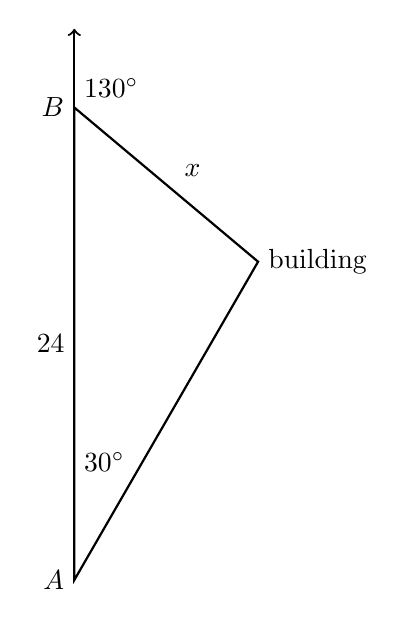
\begin{tikzpicture}[scale=0.25]
    \draw [thick]
    (-40:12.185)node[right]{building}--
    (0,0)node[left]{$B$}--
    (0,-24)node[left]{$A$}--cycle;
    \draw [thick, ->] (0,0)--(0,4);
    \node at (0,-12)[left]{$24$};
    \node at (6,-4)[above]{$x$};
    \node at (0,-18)[right]{$30^\circ$};
    \node at (0,1)[right]{$130^\circ$};
  \end{tikzpicture}
\end{center}

\item From the top of a cliff 110 m high a sailor sees two boats in the distance. One boat lies at an angle of depression of $7^\circ$ and the other at angle of depression of $15^\circ$. Given that the boats and the sailor lie in the same vertical plane, find the distance between the two boats. \hfill (6 marks)

\item A triangular field has boundaries of length 120 m, 145 m, and 155 m. 
\begin{enumerate}
  \item Find the size of the smallest interior angle of the field. \hfill (3 marks)
  \item Hence find the area of the field. \hfill (3 marks)
\end{enumerate}

\item A right triangular prism has a height of 10 cm and bases that are equilateral triangles with side length 7 cm.
\begin{enumerate}
  \item Draw a net of the prism. \hfill (2 marks)
  \item Calculate the volume of the prism. \hfill (3 marks)
  \item Calculate the total surface area of the prism. \hfill (2 marks)
\end{enumerate}

\newpage
\item A triangle field is shown with two sides measuring 70 m and 250 m. The measured sides meet at $65^\circ$ at point $A$. A horse is tied to a stake at point $A$ with a rope 70 m long so that it can graze within the sector marked. \\[0.25cm]
Find the area of the field that the horse cannot reach. \hfill (6 marks)
  \begin{center}
    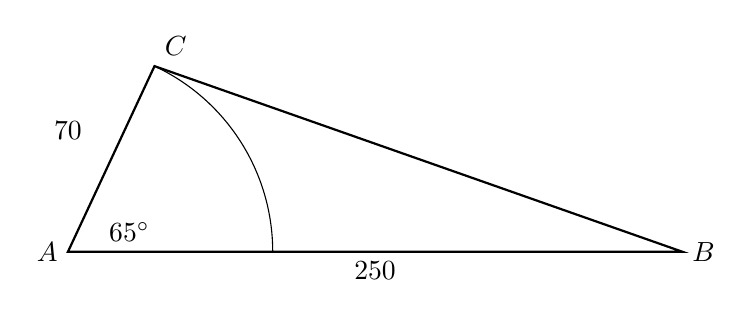
\begin{tikzpicture}[scale=1.3]
      \draw [-, thick] (65:2) node[above right]{$C$}--
        (0,0) node[left]{$A$}--
        (6,0) node[right]{$B$}--cycle;
      \draw (2,0) arc (0:65:2);
      \node at (0.6, 0)[above]{$65^\circ$};
      \node at (0, 1)[above]{$70$};
      \node at (3, 0)[below]{$250$};
    \end{tikzpicture}
    \end{center}

\item For parallel resistors in an electrical circuit, the total resistance $R_{TOT}$ is given by the formula 
$$ \frac{1}{R_{TOT}} = \frac{1}{R_1} + \frac{1}{R_2}$$
Given that the resistances of two resistors are $R_1 = 5.4 \Omega$ and $R_2 = 2.7 \Omega$, each measured to the nearest ohm.
\begin{enumerate}
  \item Find the upper and lower bounds of the total resistance. \hfill (6 marks)
  \item Given that the actual resistance of the circuit is 1.8 ohms, find the range of percentage errors that could be obtained for $R_{TOT}$. \hfill (4 marks)
\end{enumerate}

\item The following diagram shows quadrilateral $ABCD$ (not drawn to scale).
  \begin{center}
    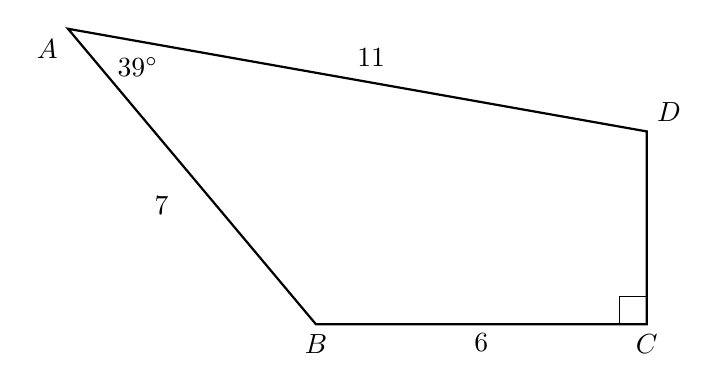
\begin{tikzpicture}[scale=0.7]
      \draw [-, thick] (130:7) node[below left]{$A$}--
        (0,0) node[below]{$B$}--
        (6,0) node[below]{$C$}--
        (6,3.5) node[above right]{$D$} -- cycle;
      \draw (6,0)++(-0.5,0)--++(0,0.5)--++(0.5,0);
      \node at (129:6)[right]{$39^\circ$};
      \node at (1,4.5)[above]{$11$};
      \node at (3,0)[below]{$6$};
      %\node at (78:3.5)[below]{$4.2$};
      \node at (-2.8,2.5)[below]{$7$};
    \end{tikzpicture}
    \end{center} 
    $AB=7$, $BC=6$, $AD=11$, $B\hat{A}D=39^\circ$, and $\overline{BC} \perp \overline{CD}$
    \begin{enumerate}
      \item Find the perimeter of the quadrilateral. \hfill [5 marks]
      \item Find the area of the quadrilateral. \hfill [3 marks]
    \end{enumerate}


\newpage
\item The pyramid $ABCDE$ has a square base with side length 15 cm. The vertex $E$ is located directly above the center of the base $ABCD$.
\begin{center}
  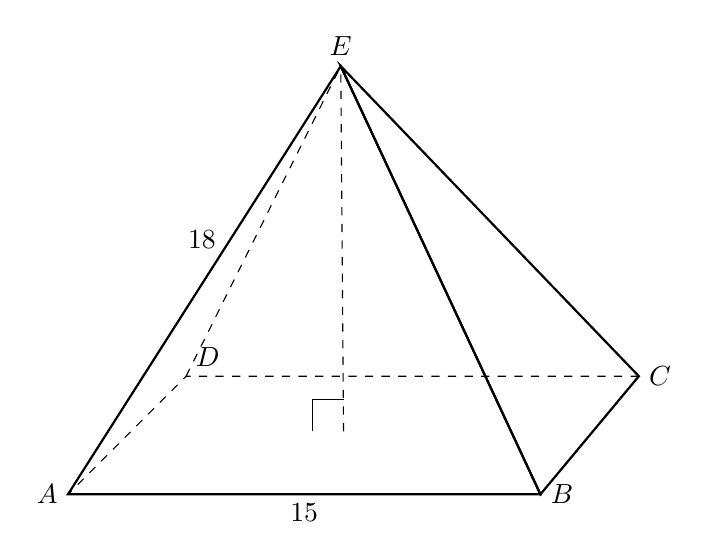
\begin{tikzpicture}[scale=1]
    \draw [-, thick] (-6,0) node[left]{$A$}--
      (0,0) node[right]{$B$}--
      (115:6) node[above]{$E$}--cycle;
    \draw [-, thick] (0,0)--
      (1.25,1.5) node[right]{$C$}--
      (115:6)--cycle;
    \draw [-, dashed] (1.25,1.5)--(-4.5,1.5)--(-6,0);
    \draw [-, dashed] (-4.5,1.5) node[above right]{$D$}--(115:6);
    \draw [-, dashed] (-2.5,0.8)--(115:6);
    \draw (-2.5,0.8)++(-0.4,0)--++(0,0.4)--++(0.4,0);
    \node at (-4,3)[above left]{$18$};
    \node at (-3,0)[below]{$15$};
  \end{tikzpicture}
  \end{center}

  $AB=15$, $AE=18$
  \begin{enumerate}
    \item Calculate the angle between the line $\overline{AE}$ and the face $ABCD$. \hfill [4 marks]
    \item Calculate the angle between the plane face $BCE$ and the face $ABCD$. \hfill [4 marks]
    \item Calculate the angle between the line $\overline{AE}$ and the line $\overline{EC}$. \hfill [2 marks]
    \item Find the volume of the pyramid. \hfill [2 marks]
    \item Find the total surface area of the pyramid, including the base. \hfill [3 marks]
  \end{enumerate}

\end{enumerate}
\end{document}
